\section{Diagrama de Use Cases}
\label{useCases}
\subsection{Diagramas}
Os Use Cases por nós apresentados e especificados na secção seguinte foram organizados em seis diagramas:

\subsubsection{Geral}
		\begin{center}
 			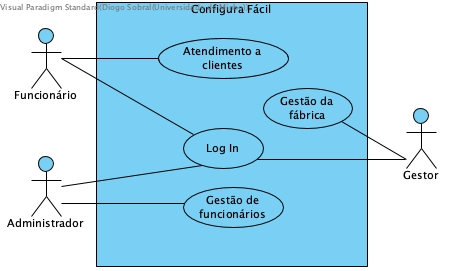
\includegraphics[scale = 0.7]{D_USECASE/Geral.jpg}
		\end{center}
\subsubsection{Gestão de Funcionários}
		\begin{center}
 			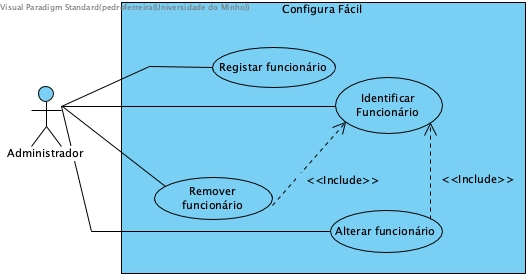
\includegraphics[scale = 0.7]{D_USECASE/Gestao_de_funcionarios.jpg}
		\end{center}\newpage
\subsubsection{Gestão de Clientes}
		\begin{center}
 			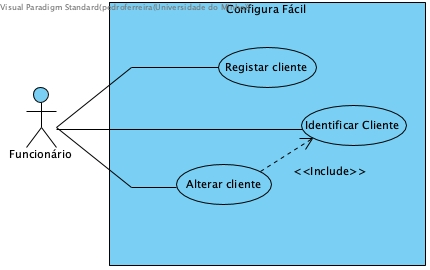
\includegraphics[scale = 0.7]{D_USECASE/Gestao_de_clientes.jpg}
		\end{center}
\subsubsection{Atendimento a Clientes}
		\begin{center}
 			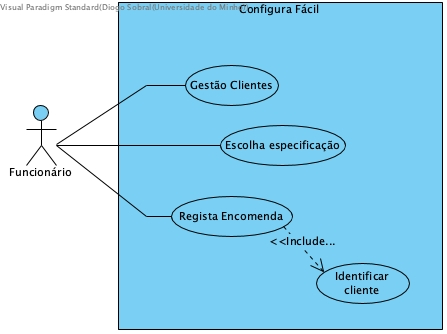
\includegraphics[scale = 0.7]{D_USECASE/Atendimento_a_clientes.jpg}
		\end{center}\newpage
\subsubsection{Escolha da Especificação}
		\begin{center}
 			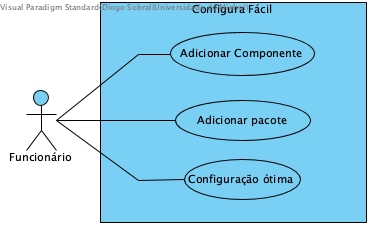
\includegraphics[scale = 0.7]{D_USECASE/Escolha_da_especificacao.jpg}
		\end{center}
\subsubsection{Gestão da Fábrica}
		\begin{center}
 			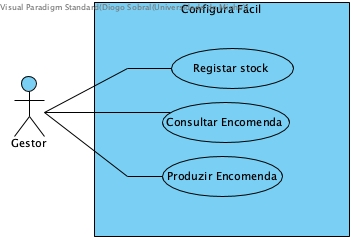
\includegraphics[scale = 0.7]{D_USECASE/Gestao_da_fabrica.jpg}
		\end{center}
\subsection{Atores}
\subsubsection{Funcionário}
Representa um funcionário do stand responsável por atender os clientes. Um funcionário tem permissões para poder gerar configurações e registar encomendas. Cabe a um funcionário a parte de gestão dos clientes.

\subsubsection{Gestor}
Representa um funcionário do stand que trabalha na parte da produção de carros. Este ator é responsável por gerir o stock e encomenda-lo. Um gestor tem acesso a todas as encomendas que ainda não foram produzidas e é este de decide qual destas deve avançar mediante o stock existente.

\subsubsection{Administrador}
Representa a pessoa do stand responsável por gerir os funcionários.

\newpage